\section{Section 3 - Smoothing}

\begin{minipage}{\linewidth}
  \begin{minipage}{0.4\linewidth}
    \begin{figure}[H]
      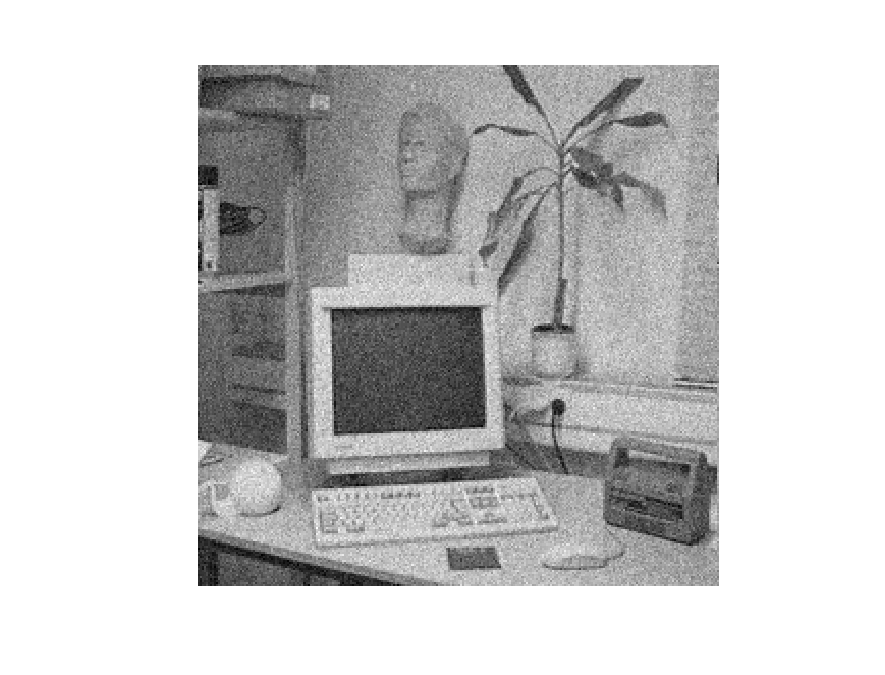
\includegraphics[scale=0.6]{./images/Q17/add_original.eps}
      \caption{Image \texttt{add}, i.e. image \texttt{office256} corrupted by white noise of $\sigma = 16$.}
      \label{fig:Q17_add_original}
    \end{figure}
  \end{minipage}
  \hspace{0.05\linewidth}
  \begin{minipage}{0.4\linewidth}
    \begin{figure}[H]
      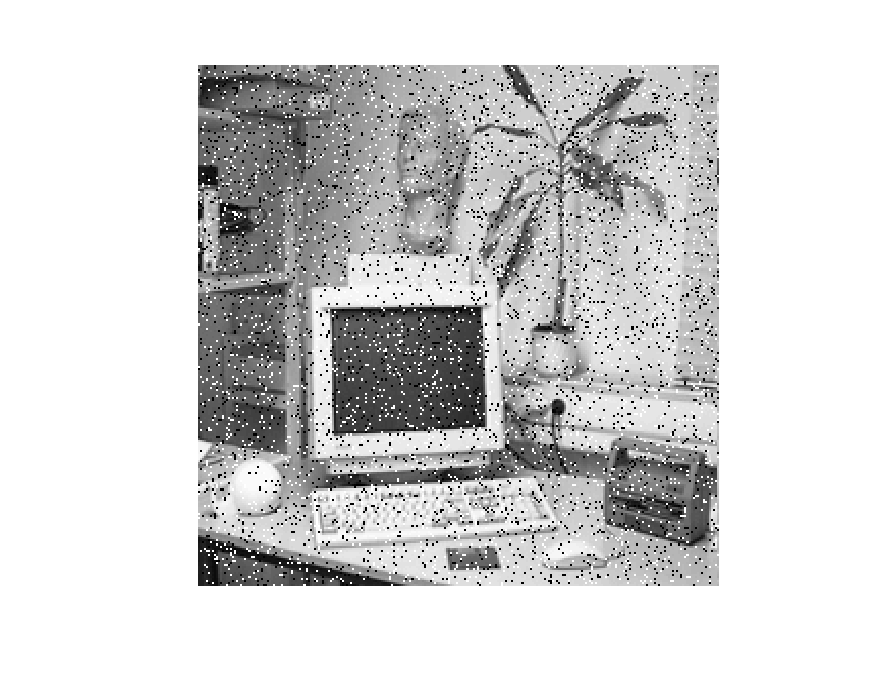
\includegraphics[scale=0.6]{./images/Q17/sap_original.eps}
      \caption{Image \texttt{sap}, i.e. \texttt{office256} corrupted by salt-and-pepper noise.}
      \label{fig:Q17_add_original}
    \end{figure}
  \end{minipage}
\end{minipage}
\\

\subsection{Question 17}

Figures \ref{fig:Q17_discgaussfft_add_01} - \ref{fig:Q17_discgaussfft_sap_10} illustrate the effect of Gaussian smoothing of images 
\texttt{add} and \texttt{sap} for various values of variance. Figures \ref{fig:Q17_medfilt_add_1} - \ref{fig:Q17_medfilt_sap_10} illustrate 
the effect of median filtering of images \texttt{add} and \texttt{sap} for various window sizes. Finally, Figures \ref{fig:Q17_ideal_add_01} -
\ref{fig:Q17_ideal_sap_005} illustrate the effect of ideal low-pass filtering of images \texttt{add} and \texttt{sap} for various cut-off frequencies.

Gaussian smoothing blurs the noise present in image \texttt{add} and as the filter's variance increases so does the disappearance of details, since
this is a type of low-pass filtering. That said, however, its behaviour in preserving details is better in terms of understanding the visual content than
the other two filters discussed here. On the other hand, Gaussian filtering integrates salt-and-pepper noise into the image, as the blurring of this type of noise
enhances it, rather than the true signal.

Median filtering has the positive property of preserving shading as is apparent in the left-hand area of the \texttt{office} image, next to the sculptured
head. Moreover, it accomplishes to eliminate in full the salt-and-pepper noise present in the \texttt{sap} image. However, this method of filtering results in
images that look like paintings, hence a substantial amount of visible information ends up being lost. This effect is more intense as the window size increases.

The ideal low-pass filter exhibits the worst behaviour regarding both types of noise. Not only does it propagate salt-and-pepper noise, but it also introduces
and propagates a noise of its own: ringing. As the cut-off frequency decreases, so do the visual details in the images. Indicatively, a cut-off frequency of 
$0.05$ cycles per pixel results in almost total corruption of the visual content of the two images.

\subsubsection{Gaussian smoothing}

\begin{minipage}{\linewidth}
  \begin{minipage}{0.4\linewidth}
    \begin{figure}[H]
      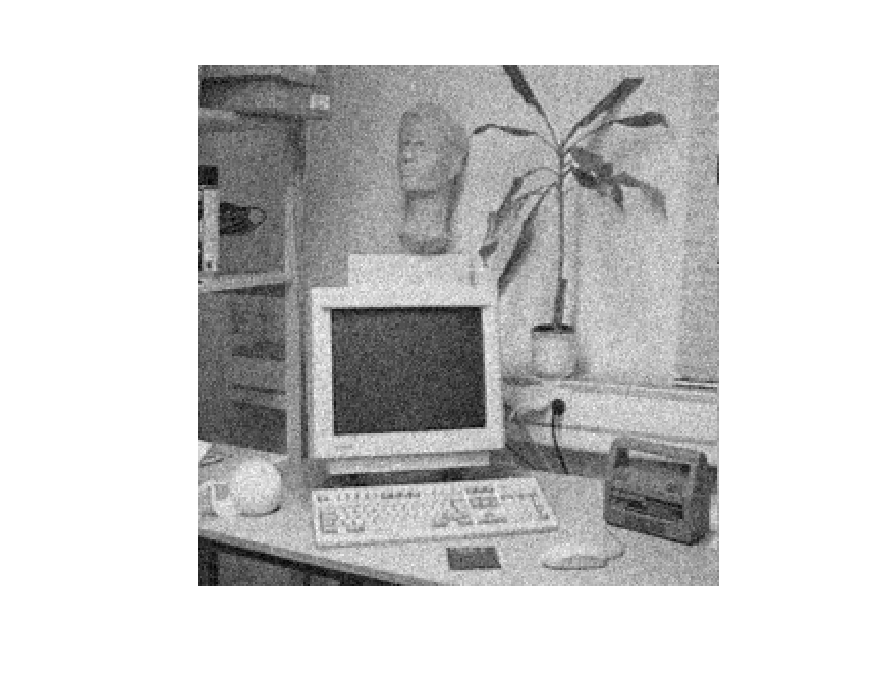
\includegraphics[scale=0.6]{./images/Q17/discgaussfft/add_01.eps}
      \caption{Smoothing of image \texttt{add} using a gaussian low pass filter of $\sigma^2 = 0.1$.}
      \label{fig:Q17_discgaussfft_add_01}
    \end{figure}
  \end{minipage}
  \hspace{0.05\linewidth}
  \begin{minipage}{0.4\linewidth}
    \begin{figure}[H]
      \includegraphics[scale=0.6]{./images/Q17/discgaussfft/add_1.eps}
      \caption{Smoothing of image \texttt{add} using a gaussian low pass filter of $\sigma^2 = 1$.}
      \label{fig:Q17_discgaussfft_add_1}
    \end{figure}
  \end{minipage}
\end{minipage}
\\

\begin{minipage}{\linewidth}
  \begin{minipage}{0.4\linewidth}
    \begin{figure}[H]
      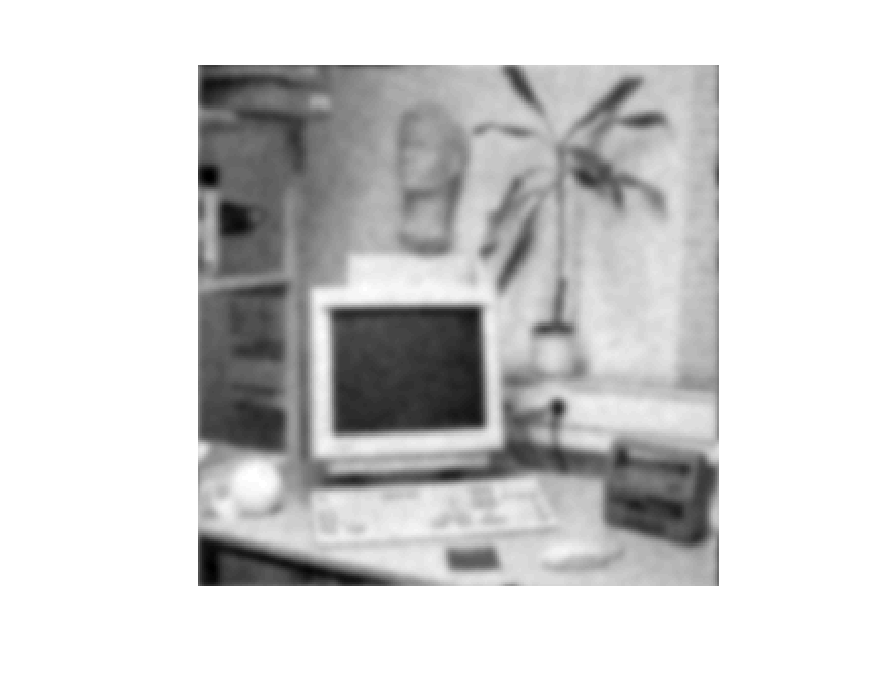
\includegraphics[scale=0.6]{./images/Q17/discgaussfft/add_4.eps}
      \caption{Smoothing of image \texttt{add} using a gaussian low pass filter of $\sigma^2 = 4$.}
      \label{fig:Q17_discgaussfft_add_4}
    \end{figure}
  \end{minipage}
  \hspace{0.05\linewidth}
  \begin{minipage}{0.4\linewidth}
    \begin{figure}[H]
      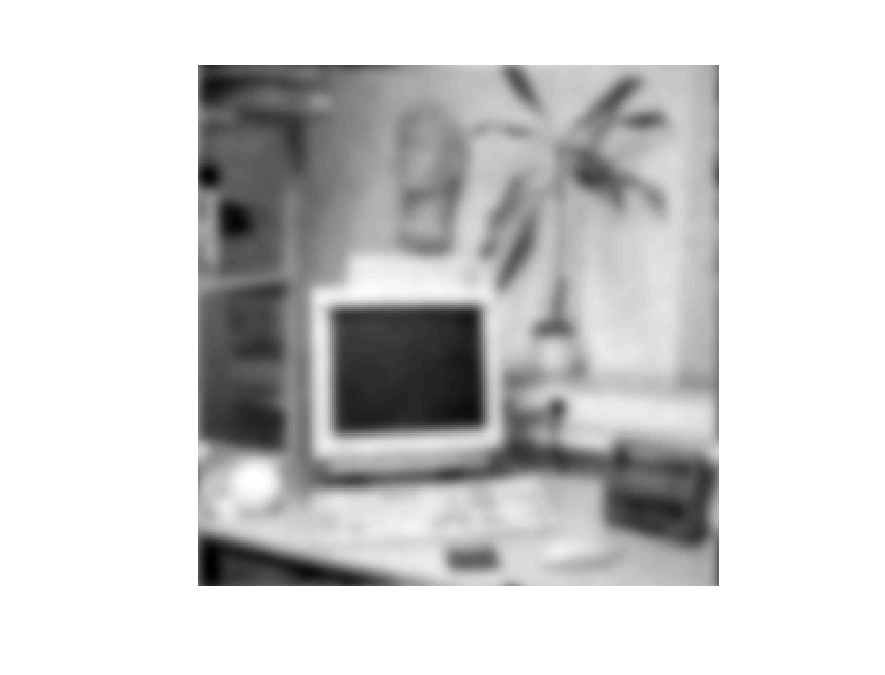
\includegraphics[scale=0.6]{./images/Q17/discgaussfft/add_10.eps}
      \caption{Smoothing of image \texttt{add} using a gaussian low pass filter of $\sigma^2 = 10$.}
      \label{fig:Q17_discgaussfft_add_10}
    \end{figure}
  \end{minipage}
\end{minipage}
\\


\begin{minipage}{\linewidth}
  \begin{minipage}{0.4\linewidth}
    \begin{figure}[H]
      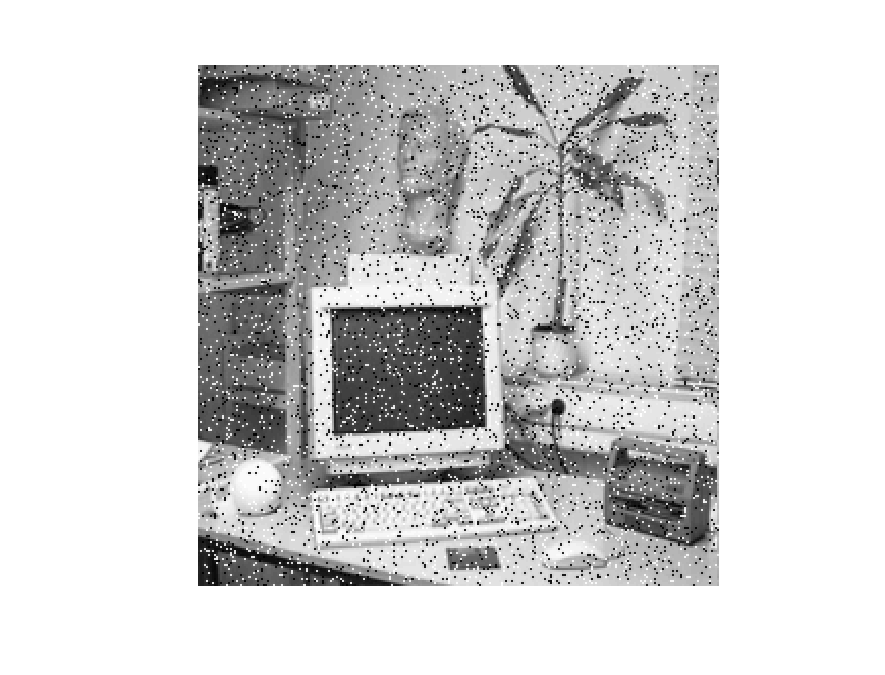
\includegraphics[scale=0.6]{./images/Q17/discgaussfft/sap_01.eps}
      \caption{Smoothing of image \texttt{sap} using a gaussian low pass filter of $\sigma^2 = 0.1$.}
      \label{fig:Q17_discgaussfft_sap_01}
    \end{figure}
  \end{minipage}
  \hspace{0.05\linewidth}
  \begin{minipage}{0.4\linewidth}
    \begin{figure}[H]
      \includegraphics[scale=0.6]{./images/Q17/discgaussfft/sap_1.eps}
      \caption{Smoothing of image \texttt{sap} using a gaussian low pass filter of $\sigma^2 = 1$.}
      \label{fig:Q17_discgaussfft_sap_1}
    \end{figure}
  \end{minipage}
\end{minipage}
\\

\begin{minipage}{\linewidth}
  \begin{minipage}{0.4\linewidth}
    \begin{figure}[H]
      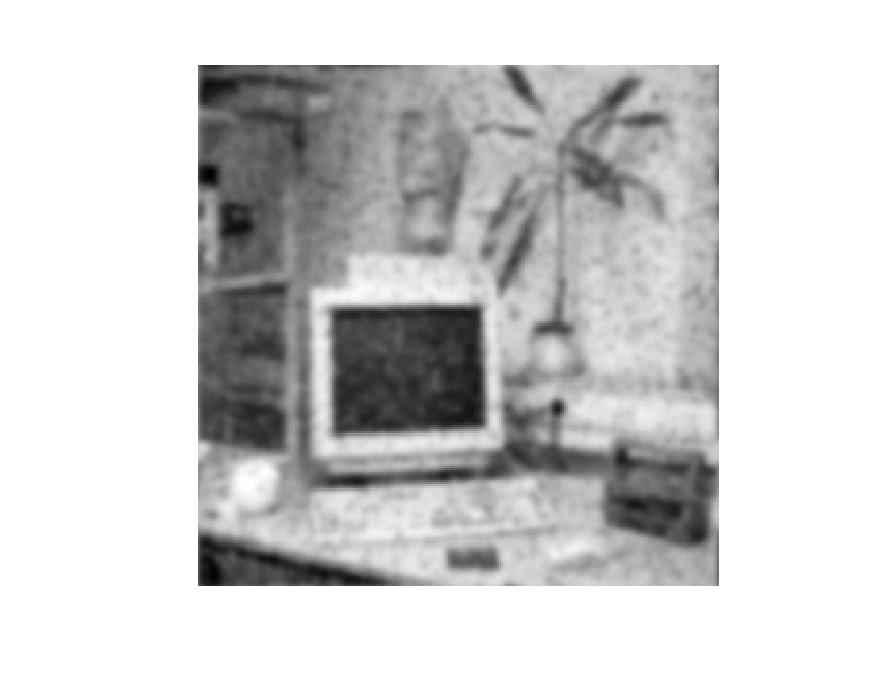
\includegraphics[scale=0.6]{./images/Q17/discgaussfft/sap_4.eps}
      \caption{Smoothing of image \texttt{sap} using a gaussian low pass filter of $\sigma^2 = 4$.}
      \label{fig:Q17_discgaussfft_sap_4}
    \end{figure}
  \end{minipage}
  \hspace{0.05\linewidth}
  \begin{minipage}{0.4\linewidth}
    \begin{figure}[H]
      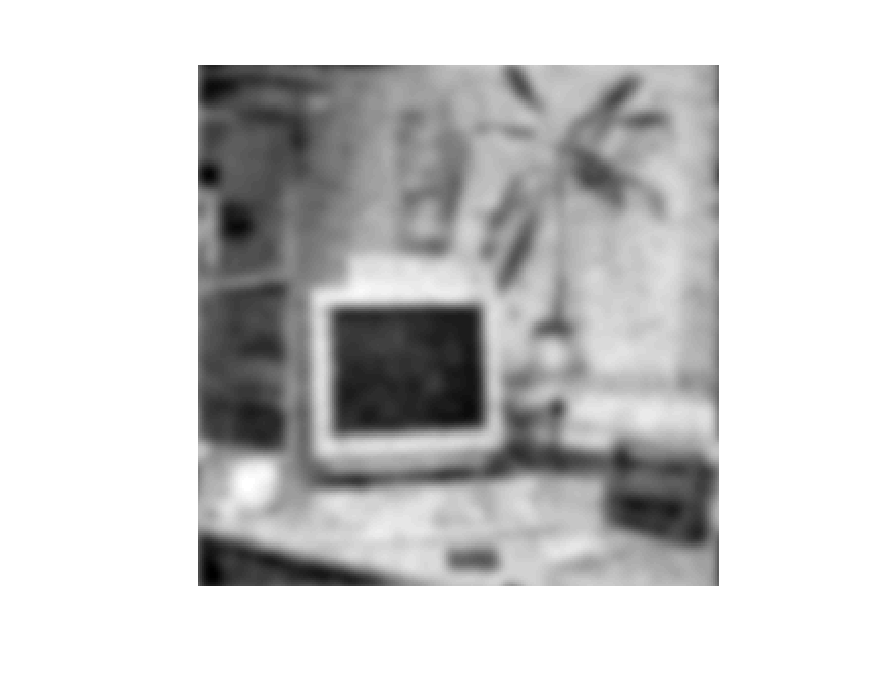
\includegraphics[scale=0.6]{./images/Q17/discgaussfft/sap_10.eps}
      \caption{Smoothing of image \texttt{sap} using a gaussian low pass filter of $\sigma^2 = 10$.}
      \label{fig:Q17_discgaussfft_sap_10}
    \end{figure}
  \end{minipage}
\end{minipage}
\\



\subsubsection{Median filtering}

\begin{minipage}{\linewidth}
  \begin{minipage}{0.4\linewidth}
    \begin{figure}[H]
      \includegraphics[scale=0.6]{./images/Q17/medfilt/add_1.eps}
      \caption{Smoothing of image \texttt{add} using a median filter of $size=1$.}
      \label{fig:Q17_medfilt_add_1}
    \end{figure}
  \end{minipage}
  \hspace{0.05\linewidth}
  \begin{minipage}{0.4\linewidth}
    \begin{figure}[H]
      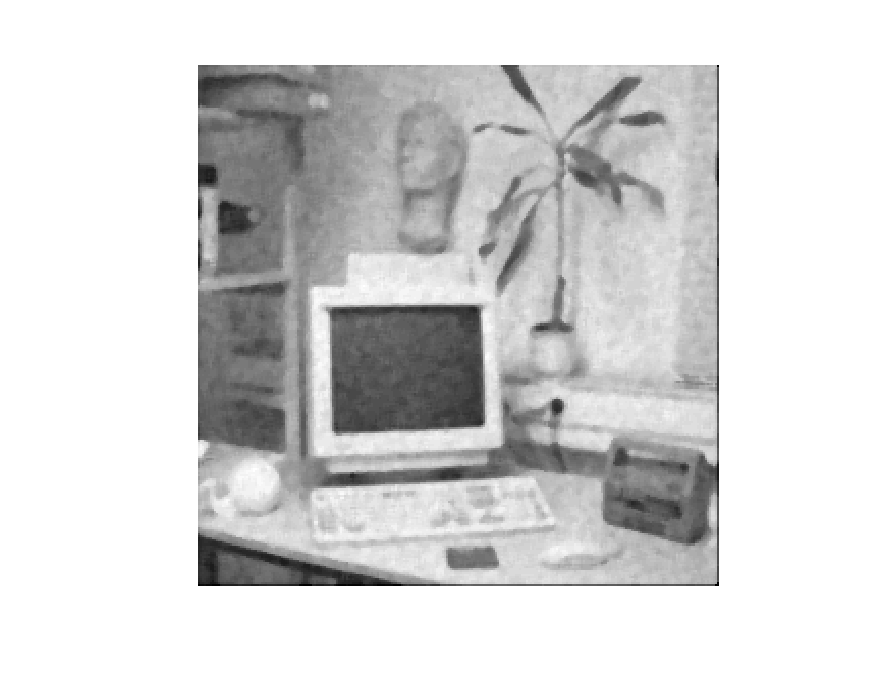
\includegraphics[scale=0.6]{./images/Q17/medfilt/add_4.eps}
      \caption{Smoothing of image \texttt{add} using a median filter of $size=4$.}
      \label{fig:Q17_medfilt_add_4}
    \end{figure}
  \end{minipage}
\end{minipage}
\\

\begin{minipage}{\linewidth}
  \begin{minipage}{0.4\linewidth}
    \begin{figure}[H]
      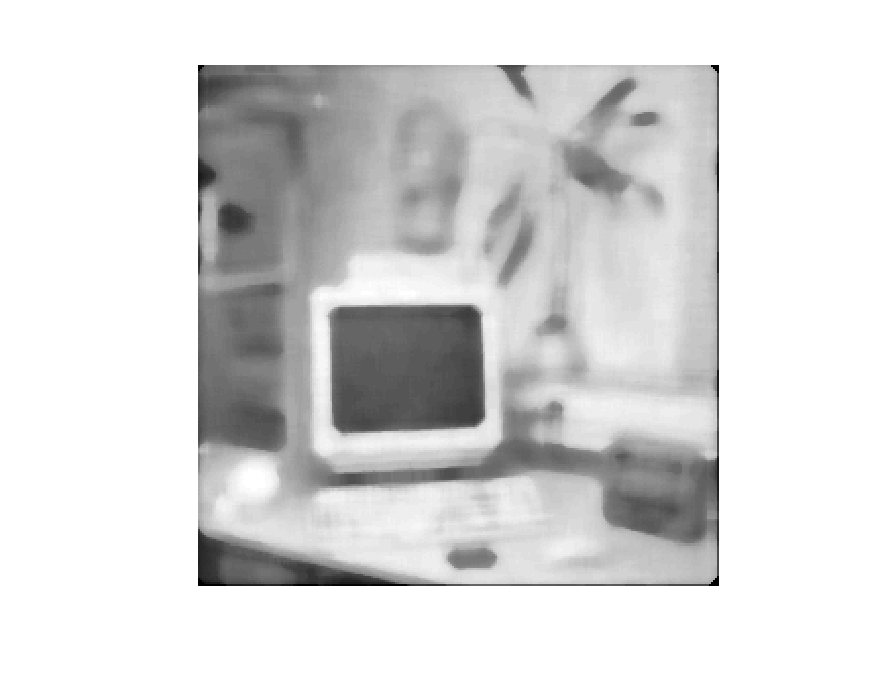
\includegraphics[scale=0.6]{./images/Q17/medfilt/add_10.eps}
      \caption{Smoothing of image \texttt{add} using a median filter of $size=10$.}
      \label{fig:Q17_medfilt_add_10}
    \end{figure}
  \end{minipage}
  \hspace{0.05\linewidth}
  \begin{minipage}{0.4\linewidth}
    \begin{figure}[H]
      \includegraphics[scale=0.6]{./images/Q17/medfilt/sap_1.eps}
      \caption{Smoothing of image \texttt{sap} using a median filter of $size=1$.}
      \label{fig:Q17_medfilt_sap_1}
    \end{figure}
  \end{minipage}
\end{minipage}
\\


\begin{minipage}{\linewidth}
  \begin{minipage}{0.4\linewidth}
    \begin{figure}[H]
      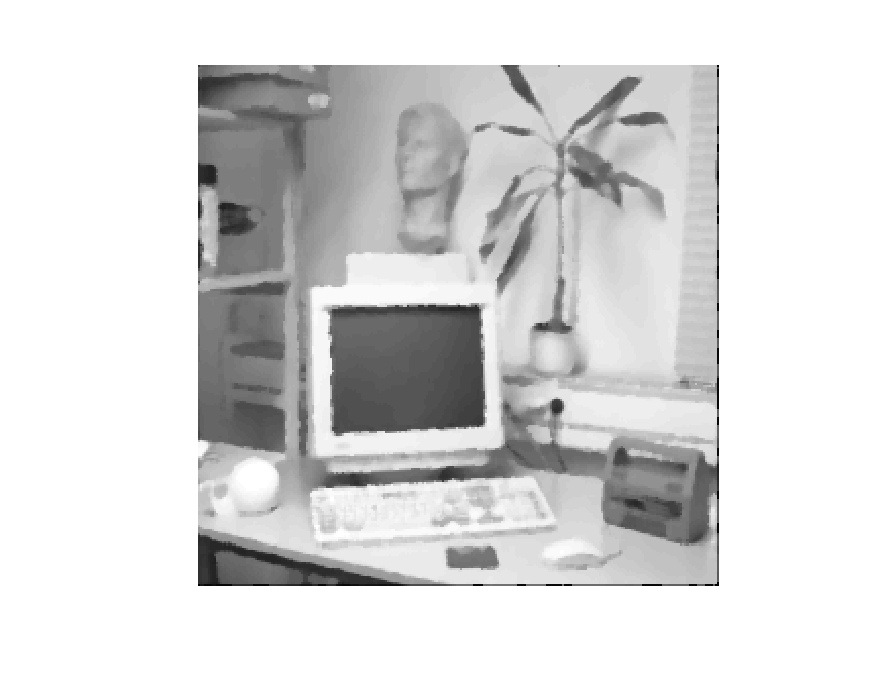
\includegraphics[scale=0.6]{./images/Q17/medfilt/sap_4.eps}
      \caption{Smoothing of image \texttt{sap} using a median filter of $size=4$.}
      \label{fig:Q17_medfilt_sap_4}
    \end{figure}
  \end{minipage}
  \hspace{0.05\linewidth}
  \begin{minipage}{0.4\linewidth}
    \begin{figure}[H]
      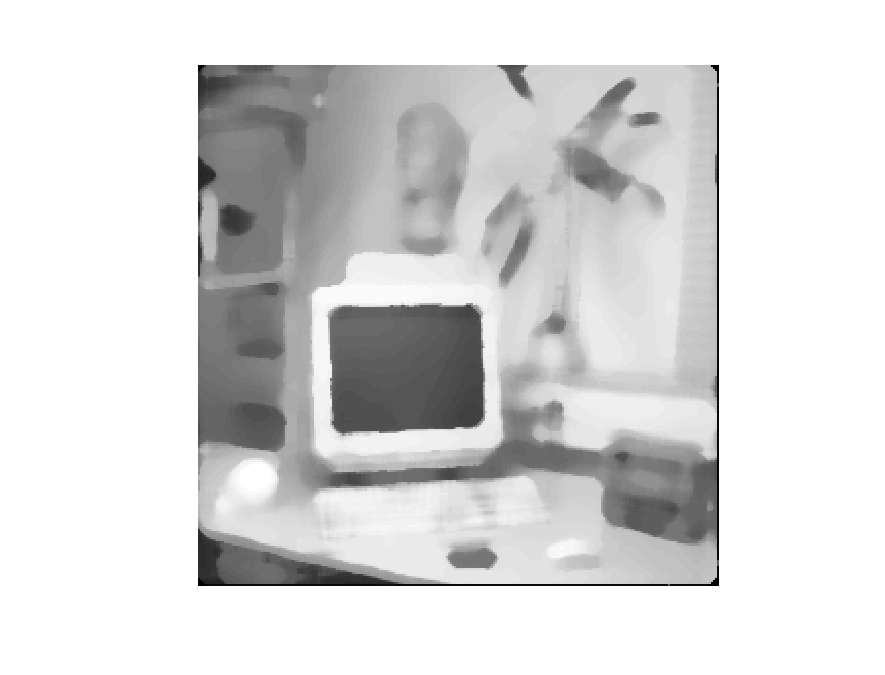
\includegraphics[scale=0.6]{./images/Q17/medfilt/sap_10.eps}
      \caption{Smoothing of image \texttt{sap} using a median filter of $size=10$.}
      \label{fig:Q17_medfilt_sap_10}
    \end{figure}
  \end{minipage}
\end{minipage}
\\



\subsubsection{Ideal low-pass filtering}

\begin{minipage}{\linewidth}
  \begin{minipage}{0.4\linewidth}
    \begin{figure}[H]
      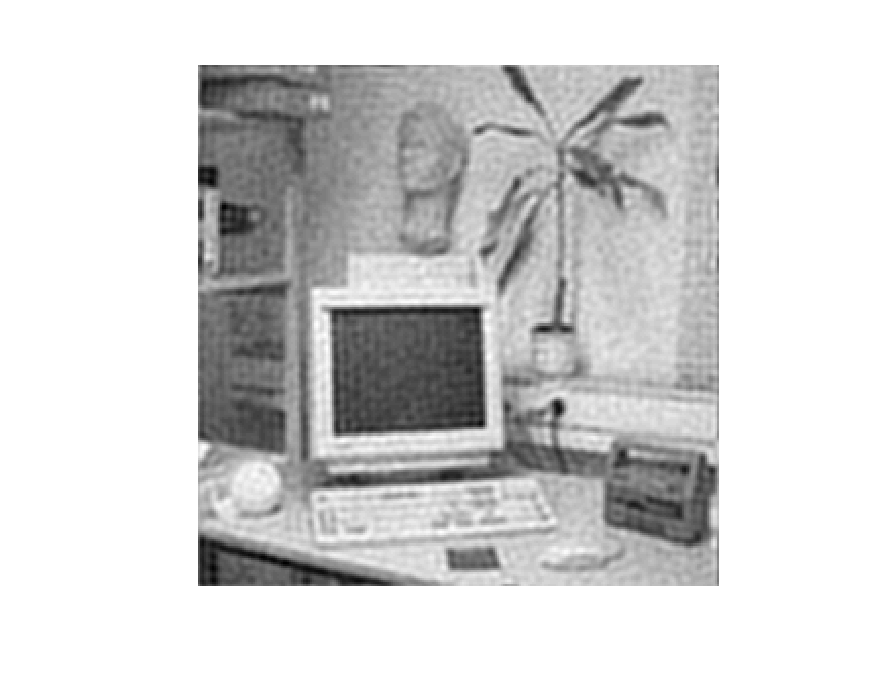
\includegraphics[scale=0.5]{./images/Q17/ideal/add_02.eps}
      \caption{Smoothing of image \texttt{add} using an ideal low-pass filter with cut-off frequency of $0.2$ cycles per pixel.}
      \label{fig:Q17_ideal_add_02}
    \end{figure}
  \end{minipage}
   \begin{minipage}{0.4\linewidth}
    \begin{figure}[H]
      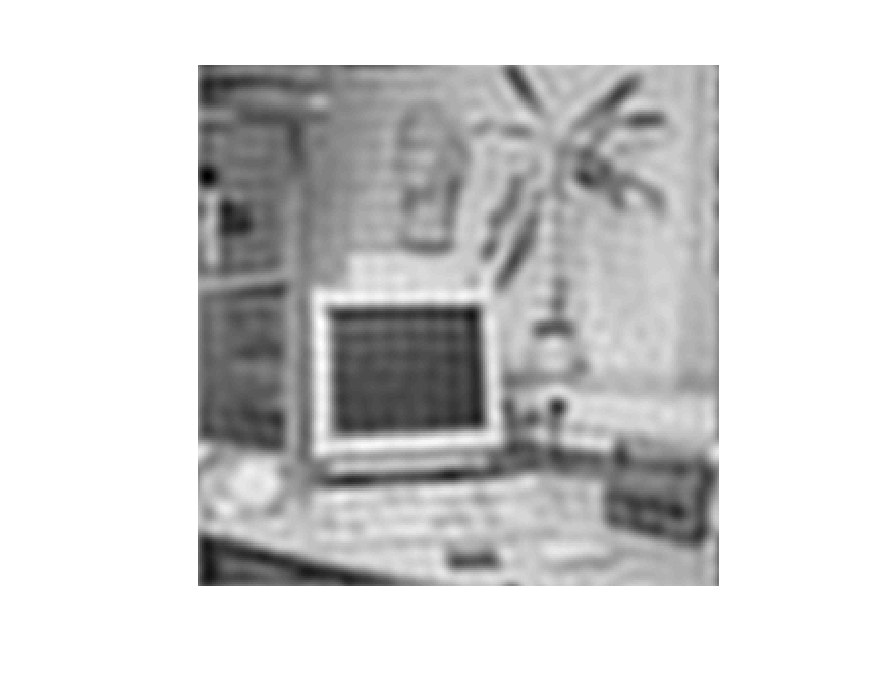
\includegraphics[scale=0.5]{./images/Q17/ideal/add_01.eps}
      \caption{Smoothing of image \texttt{add} using an ideal low-pass filter with cut-off frequency of $0.1$ cycles per pixel.}
      \label{fig:Q17_ideal_add_01}
    \end{figure}
  \end{minipage}
  \hspace{0.05\linewidth}
\end{minipage}
\\

\begin{minipage}{\linewidth}
  \begin{minipage}{0.4\linewidth}
    \begin{figure}[H]
      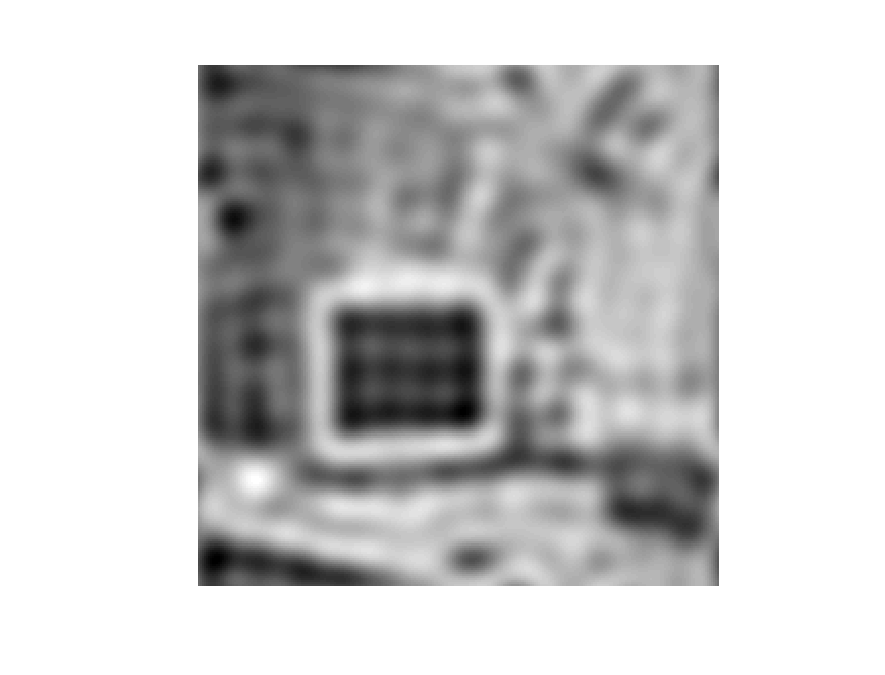
\includegraphics[scale=0.5]{./images/Q17/ideal/add_005.eps}
      \caption{Smoothing of image \texttt{add} using an ideal low-pass filter with cut-off frequency of $0.05$ cycles per pixel.}
      \label{fig:Q17_ideal_add_005}
    \end{figure}
  \end{minipage}
  \hspace{0.05\linewidth}
   \begin{minipage}{0.4\linewidth}
    \begin{figure}[H]
      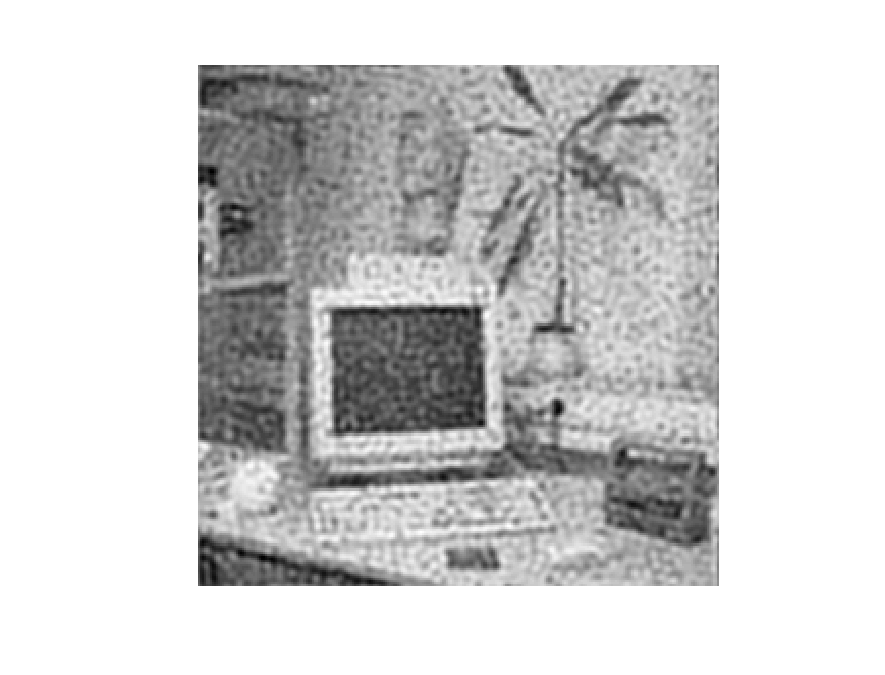
\includegraphics[scale=0.5]{./images/Q17/ideal/sap_02.eps}
      \caption{Smoothing of image \texttt{sap} using an ideal low-pass filter with cut-off frequency of $0.2$ cycles per pixel.}
      \label{fig:Q17_ideal_sap_02}
    \end{figure}
  \end{minipage}

\end{minipage}
\\


\begin{minipage}{\linewidth}
  \begin{minipage}{0.4\linewidth}
    \begin{figure}[H]
      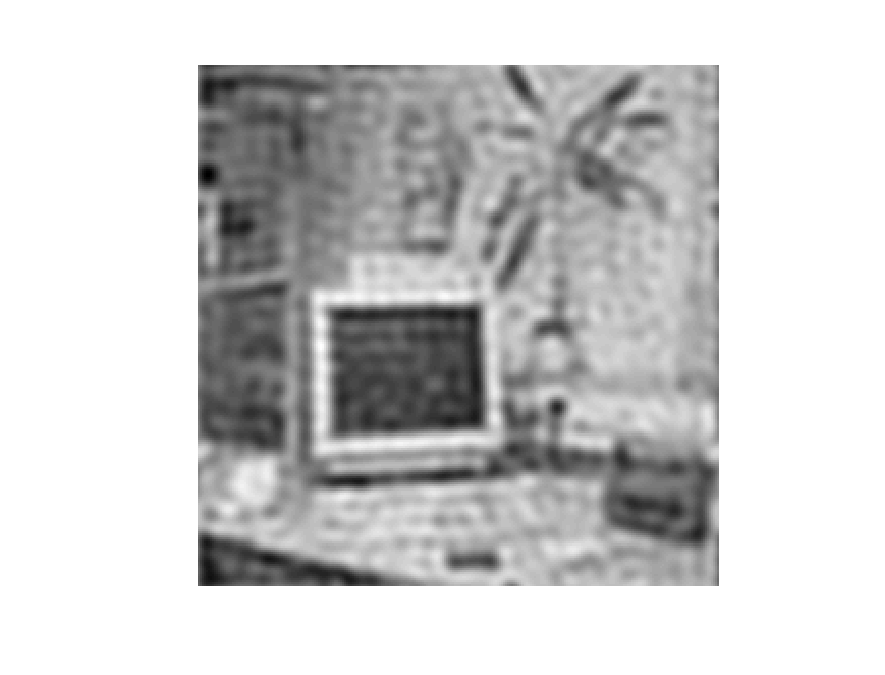
\includegraphics[scale=0.5]{./images/Q17/ideal/sap_01.eps}
      \caption{Smoothing of image \texttt{sap} using an ideal low-pass filter with cut-off frequency of $0.1$ cycles per pixel.}
      \label{fig:Q17_ideal_sap_01}
    \end{figure}
  \end{minipage}
  \hspace{0.05\linewidth}
  \begin{minipage}{0.4\linewidth}
    \begin{figure}[H]
      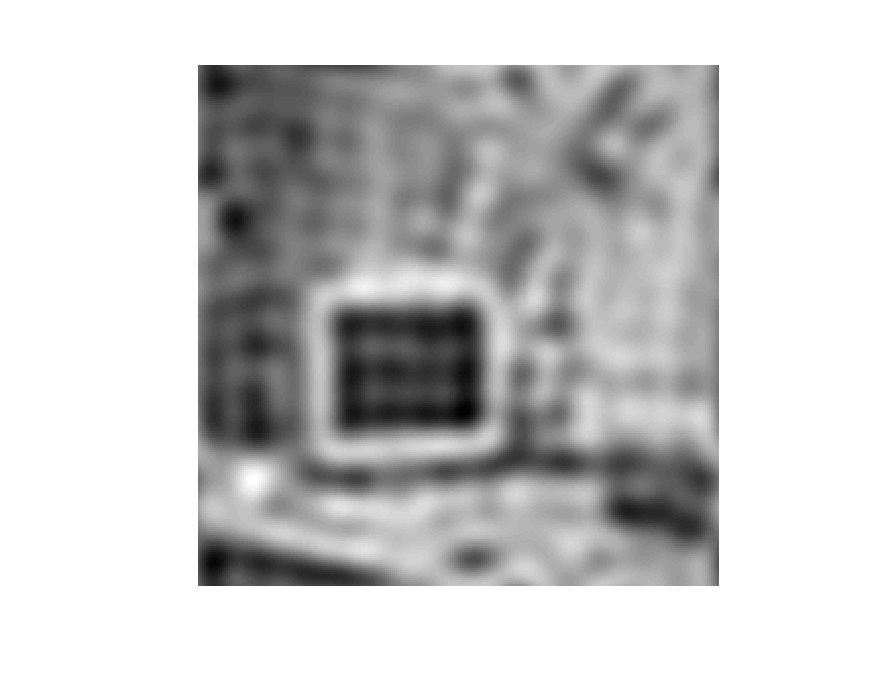
\includegraphics[scale=0.5]{./images/Q17/ideal/sap_005.eps}
      \caption{Smoothing of image \texttt{sap} using an ideal low-pass filter with cut-off frequency of $0.05$ cycles per pixel.}
      \label{fig:Q17_ideal_sap_005}
    \end{figure}
  \end{minipage}
\end{minipage}
\\


\subsection{Question 18}

With regard to the Gaussian filter, we observed that when its variance increases, so does the blurring. This is reasonable since in the frequency domain the 
variance of the filter is the inverse of the one we use. That means that the higher the variance in the spatial domain, the lower the variance in the frequency
domain. The lower the variance in the frequency domain, the more high frequencies are discarded. Hence only noise of relatively lower frequency remains present
in the image.

The ideal low-pass filter can be seen as a perfect disc with radius $r=D_0$ in the frequency domain. In the spatial domain, this filter is represented however
by two components. An intense component in the origin and a component comprised by concentric circles around the first component. The first component is
responsible for the blurring and the second one for the ringing effect. The lower the cut-off frequency, the higher the more this ringing effect is spread, that is,
the ringing effect of each pixel reaches longer distances. Since a multiplication of the Fourier transform of two signals in the frequency domain is equivalent of
a convolution in the spatial domain, the above latter component affects the filtered image in a way such that noise is not only maintained but 
also transformed. For instance, salt-and-pepper noise in the \texttt{sap} image is enhanced and magnified, resulting in large freckle-like shapes in the image.

In contrast to the two low-pass filters, the median filter is a non-linear filter whose operations are centred only on a neighbourhood. As the filter works
with the median of a neighbourhood of pixels, and not the mean, it can directly remove the effect that outliers have in images, that is, small regions of pixels 
infected by noise. The above two reasons are the reasons why this filter is so successful in removing salt-and-pepper noise.

